\begin{landscape}
    \chapter{Vývoj latentního prostoru naučeného modelu skrze různý počet epoch}
    \label{app:latent_space_development}

    \begin{figure}[H]
        \centering
        \subfloat[\centering label 1]{{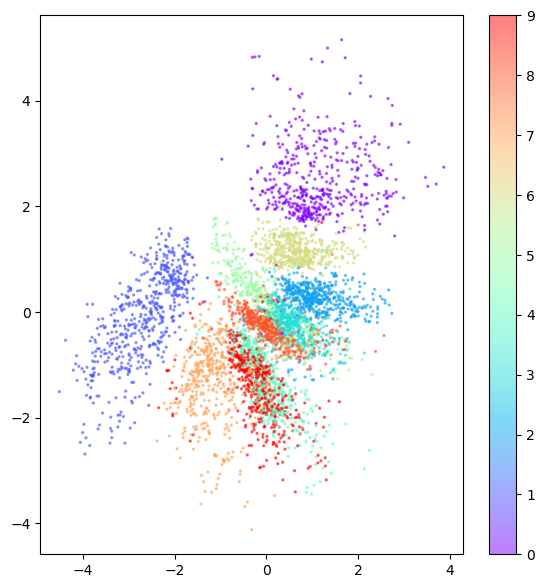
\includegraphics[width=0.50\textwidth]{figures/latent_space_200_epochs.png} }}%
        \subfloat[\centering label 2]{{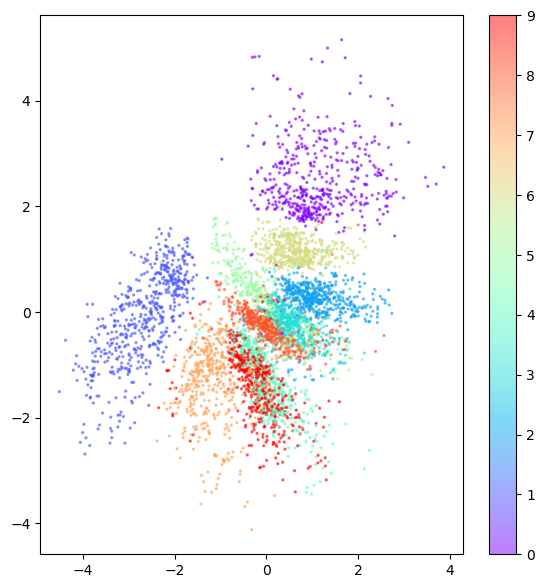
\includegraphics[width=0.50\textheight]{figures/latent_space_200_epochs.png} }}%
        \subfloat[\centering label 3]{{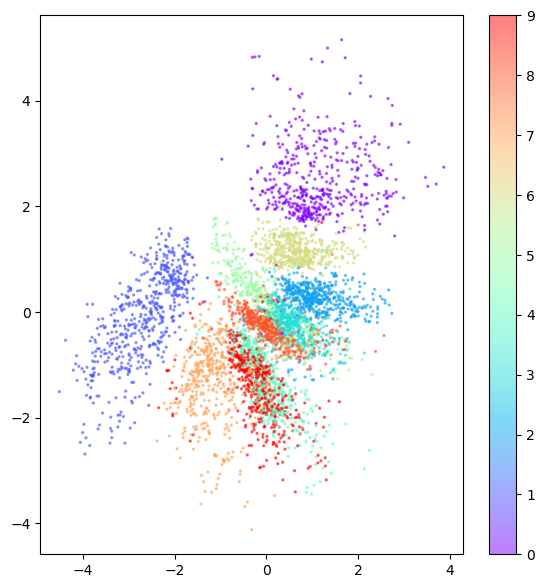
\includegraphics[width=0.50\textheight]{figures/latent_space_200_epochs.png} }}%
        \caption{2 Figures side by side}%
        \label{fig:example}%
    \end{figure}

\end{landscape}